\chapter{Cross-Validation}

\begin{wrapfigure}{o}{0.6\textwidth}
    \vspace{-0.5cm}
    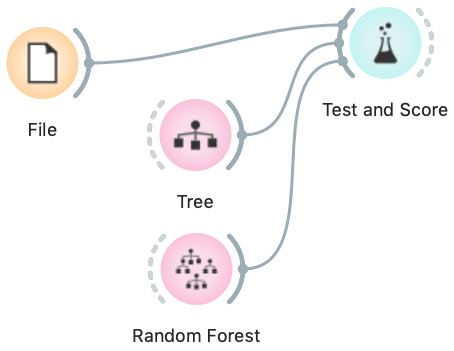
\includegraphics[scale=0.4]{workflow.png}
\end{wrapfigure}

Estimating the accuracy may depend on a particular split of the data set. To increase robustness, we can repeat the measurement several times, each time choosing a different subset of the data for training. One such method is cross-validation. It is available in Orange in the \widget{Test and Score} widget.

Note that in each iteration, \widget{Test and Score} will pick a part of the data for training, learn the predictive model on this data using some machine learning method, and then test the accuracy of the resulting model on the remaining, test data set. For this, the widget will need on its input a data set from which it will sample the data for training and testing, and a learning method which it will use on the training data set to construct a predictive model. In Orange, the learning method is simply called a learner. Hence, \widget{Test and Score} needs a learner on its input. \marginnote{For geeks: a learner is an object that, given the data, outputs a classifier. Just what \widget{Test and Score} needs.}

This is another way to use the \widget{Tree} widget. In the workflows from the previous lessons we have used another of its outputs, called \textit{Model}; its construction required data. This time, no data is needed for \widget{Tree}, because all that we need from it is a \textit{Learner}.

\begin{figure}[h]
    \centering
    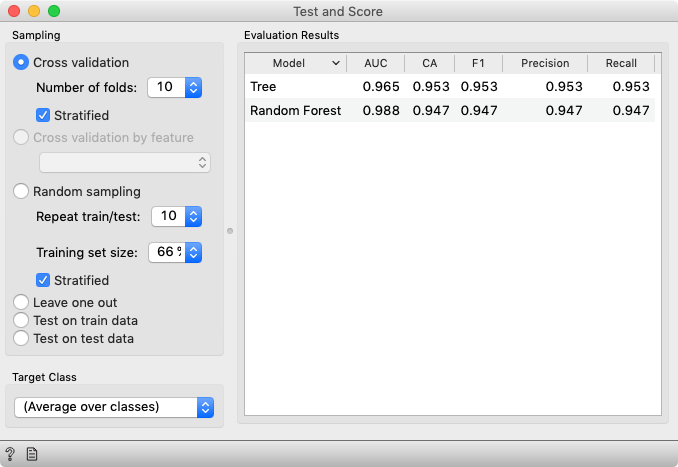
\includegraphics[scale=0.4]{test_and_score.png}
    \caption{Cross validation splits the data sets into, say, 10 different non-overlapping subsets we call folds. In each iteration, one fold will be used for testing, while the data from all other folds will be used for training. In this way, each data instance will be used for testing exactly once.}
\end{figure}

In the \widget{Test and Score} widget, the second column, CA, stands for classification accuracy, and this is what we really care for for now.